\documentclass[tikz,border=2pt]{standalone}
\usepackage{amsmath}
\usepackage{pgfplots}
\pgfplotsset{compat=1.18}
\usetikzlibrary{arrows.meta}
\begin{document}
% (x+1)^2 and (x-1)^2: their maximum (|x|+1)^2 is convex, its epigraph (shaded) is the intersection of the two epigraphs;
% their minimum has the zeros -1 and 1 but value 1 at the midpoint 0, above the chord at height 0 (Example 3: not convex).
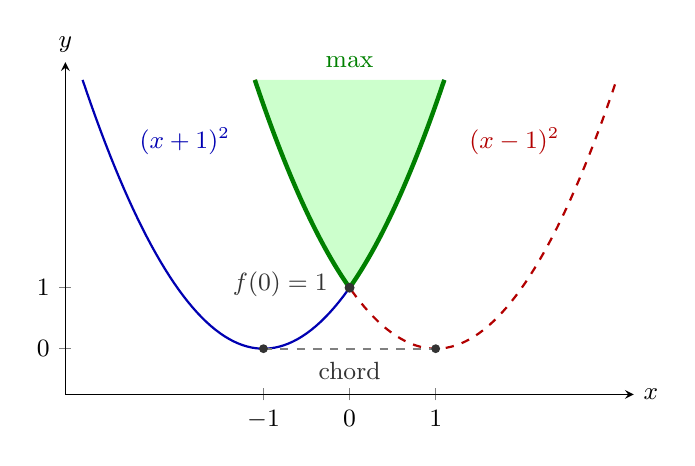
\begin{tikzpicture}[font=\small, >={Latex[length=2mm]}]
  \begin{axis}[
    axis lines=left, xmin=-3.3, xmax=3.3, ymin=-0.75, ymax=4.7,
    xtick={-1,0,1}, ytick={0,1},
    xlabel={$x$}, ylabel={$y$},
    xlabel style={at={(axis description cs:1,0)}, anchor=west},
    ylabel style={rotate=-90, at={(axis description cs:0,1)}, anchor=south},
    width=8.8cm, height=5.8cm, clip=false
    ]
    \addplot[draw=none, fill=green!20, domain=-1.1:1.1, samples=81] {(abs(x)+1)^2} -- (axis cs:1.1,4.41) -- cycle;
    \addplot[blue!70!black, thick, domain=-3.1:1.1, samples=80] {(x+1)^2};
    \addplot[red!70!black, thick, dashed, domain=-1.1:3.1, samples=80] {(x-1)^2};
    \addplot[green!50!black, ultra thick, domain=-1.1:1.1, samples=81] {(abs(x)+1)^2};
    \node[blue!70!black, anchor=west] at (axis cs:-2.55,3.4) {$(x+1)^2$};
    \node[red!70!black, anchor=east] at (axis cs:2.55,3.4) {$(x-1)^2$};
    \node[green!50!black, anchor=south] at (axis cs:0,4.45) {$\max$};
    \draw[gray, thick, dashed] (axis cs:-1,0) -- (axis cs:1,0);
    \fill[gray!40!black] (axis cs:-1,0) circle (1.6pt);
    \fill[gray!40!black] (axis cs:1,0) circle (1.6pt);
    \fill[gray!40!black] (axis cs:0,1) circle (1.8pt);
    \node[gray!40!black, anchor=north] at (axis cs:0,-0.06) {chord};
    \node[gray!40!black, anchor=east] at (axis cs:-0.14,1.06) {$f(0)=1$};
  \end{axis}
\end{tikzpicture}
\end{document}
